\section{Surface brightness and galaxy shapes}
\label{sec:fit_light}

This section focuses on the significance of fitting surface brightness models to simulated/observational data within the context of weak lensing.
Accurate modeling of surface brightness profiles is of utmost importance for the analysis of weak lensing effects.

Fitting surface brightness profiles is a crucial step in weak lensing studies for several reasons. First, it allows astronomers to precisely measure the shapes and orientations of galaxies, which can be subtly distorted by the gravitational lensing effect of foreground mass distributions. These distortions, although weak and difficult to detect, carry invaluable information about the mass distribution of the lensing objects, including dark matter, which is otherwise invisible. By analyzing the statistical alignment and shape changes of background galaxies, researchers can map the mass distribution of the lensing structures, offering insights into the nature of dark matter and the large-scale structure of the Universe.

Moreover, accurate fitting of surface brightness profiles helps in separating the lensing signal from intrinsic alignments and other observational effects, enhancing the reliability of weak lensing measurements. This process is fundamental in cosmology as it contributes to the precision modeling of the Universe's expansion and the distribution of matter on cosmic scales. Thus, the methodological advancements in fitting these profiles not only refine our understanding of individual galaxy structures but also bolster the broader applications of weak lensing as a tool for probing the fundamental components and dynamics of the cosmos.

By fitting observed surface brightness profiles with theoretical models, the ellipticity and orientation of galaxy images can be precisely determined, allowing for the reconstruction of the lensing field and the mapping of the mass distribution along the line of sight.


\subsection{Fit of Sérsic profile of surface brightness}
\label{subsec:sersic_fit}

The simulated galaxy is generated from a theoretical model, incorporating noise and applying a Point Spread Function (PSF), assuming that the sky background has already been subtracted from the image.

Incorporating noise into these simulations mimics the real observational conditions faced in astronomy. Sources of noise include detection equipment, atmospheric interference in ground-based observations, and intrinsic astronomical sources of variability. By integrating noise into the simulations, the fitting algorithms are tested for robustness, ensuring they can navigate the real-world data complexities.

Additionally, applying a Point Spread Function (PSF) is crucial. The PSF models the imaging system's response, capturing the effects of the telescope, detectors, and atmosphere that may blur and distort observed images. This is particularly relevant in the context of weak lensing because the PSF anisotropies can mimic lensing-induced ellipticities, biasing the shear measurements. Simulating these effects allows the fitting algorithms to consider them when analyzing objects' surface brightness.

We assume that the sky background has been subtracted from the image. This step isolates the light from the astronomical object from ambient environmental light, including atmospheric light, scattered light from nearby stars, and the Milky Way's diffuse glow. Precise background subtraction is essential for accurate surface brightness measurements.

The most common type of parametric surface brightness model is the Sérsic profile, which, as described in \cref{subsec:sersic}, is characterized by an exponential form. This is the usual profile adopted to represent the luminosity distribution of various astronomical objects, such as galaxies, by providing a flexible mathematical framework that describes a wide range of shapes from disk-like to elliptical structures.

The Sérsic profile is expressed mathematically as follows:
\be
\label{eq:5.1}
I(R) = I_e \exp \bc{- b_n \bs{\bp{\frac{R}{R_{e}}}^{\frac{1}{n}} - 1}} \,.
\ee

Assuming $q$ is the axis ratio of the elliptical distribution, the elliptical radius $R$ is thus
\be
\label{eq:5.2}
R = \sqrt{x_r^2 + (y_r / q)^2} \,,
\ee
where $x_r$ and $y_r$ the rotated coordinates obtained by aligning the reference frame $(x,y)$ of the observer to the axes of the ellipse
\begin{equation}
\begin{aligned}
    \label{eq:5.3}
    x_r & = (x - x_0) \cos{\varphi} + (y - y_0) \sin{\varphi} \,,
    \\
    y_r & = (y - y_0) \cos{\varphi} - (x-x_0) \sin{\varphi}  \,,
\end{aligned}
\end{equation}
where $x_0$ and $y_0$ represent the coordinates of the center of the ellipse and $\varphi$ the position angle.

Optimizing the Sérsic profile means fitting its seven parameters ($I_e$, $R_e$, $n$, $x_0$, $y_0$, $q$, $\varphi$) to observational data, which requires careful consideration of the effects of instrumental and observational factors, such as the Point Spread Function (PSF).

\subsubsection{Simulation of observational data}

The first step consists of simulating the observational data. It is done by constructing a $(x,y)$ grid on the sky plane with dimensions $\SI{100}{\arcsecond} \times \SI{100}{\arcsecond}$, with a pixel scale of $\SI{0.03}{\arcsecond\per\pixel}$.

The model for simulating the galaxy light profile and the parameters needed to create the mock data are then defined. The intensity at the effective radius, $I_e$, is expressed in arbitrary units, while the effective radius $R_e$ is expressed in arcseconds, together with the center coordinates. Furthermore, the axis ratio $q$ and position angle $\varphi$ of the galaxy are defined. They are linked to the ellipticity components $e_1$ and $e_2$ by the following relations
\begin{equation}
\begin{aligned}
    \label{eq:e1e2}
    e_1 & = \frac{1 - q}{1 + q} \cos{(2\varphi)} \,,
    \\
    e_2 & = \frac{1 - q}{1 + q} \sin{(2\varphi)}  \,,
\end{aligned}
\end{equation}
and their combination gives the ellipticity of the object
\be
\label{eq:ellip}
e = \sqrt{e_1^2 + e_2^2} = \frac{1-q}{1+q} \,.
\ee

The ellipticity is related to the semi-major and semi-minor axes, which is reflected in terms of shear. In particular, it can be demonstrated that the ellipticity coincides with the reduced shear $g$:
\be
\label{eq:red_shear}
e \equiv g = \frac{\g}{1 - \k} \,.
\ee

This is the concept at the basis of weak lensing: by measuring the ellipticity of the lensed images of background sources, we can infer the lenses' mass distribution. Given that ellipticity measures shear and convergence, it is then related to the second derivatives of the lensing potential.


We can then proceed with inserting the parameters inside the model. \Cref{tab:parameters_1} report a summary of the parameters to which the model is initialized.

When the parameters are added to the model, the theoretical observational data is produced and is shown in \cref{fig:0_clean}. Additionally, in \cref{fig:0_flux}, the theoretical Sérsic profile is shown: the surface brightness as a function of distance from the galaxy center, in units of $R_e$. Subsequently, to enhance the realism of the observational model, a Gaussian noise component with mean $\m = 0.0$ and standard deviation $\s = 0.05$ was added to the image. Furthermore, the resulting surface brightness was convolved with a Point Spread Function (PSF) characterized by a Full Width at Half Maximum (FWHM) of $\SI{0.1}{\arcsecond}$. The final ``noisy'' surface brightness profile is illustrated in \cref{fig:0_noisy}.

\begin{figure}
  \begin{minipage}{\linewidth}
    \centering
    \subfloat[]{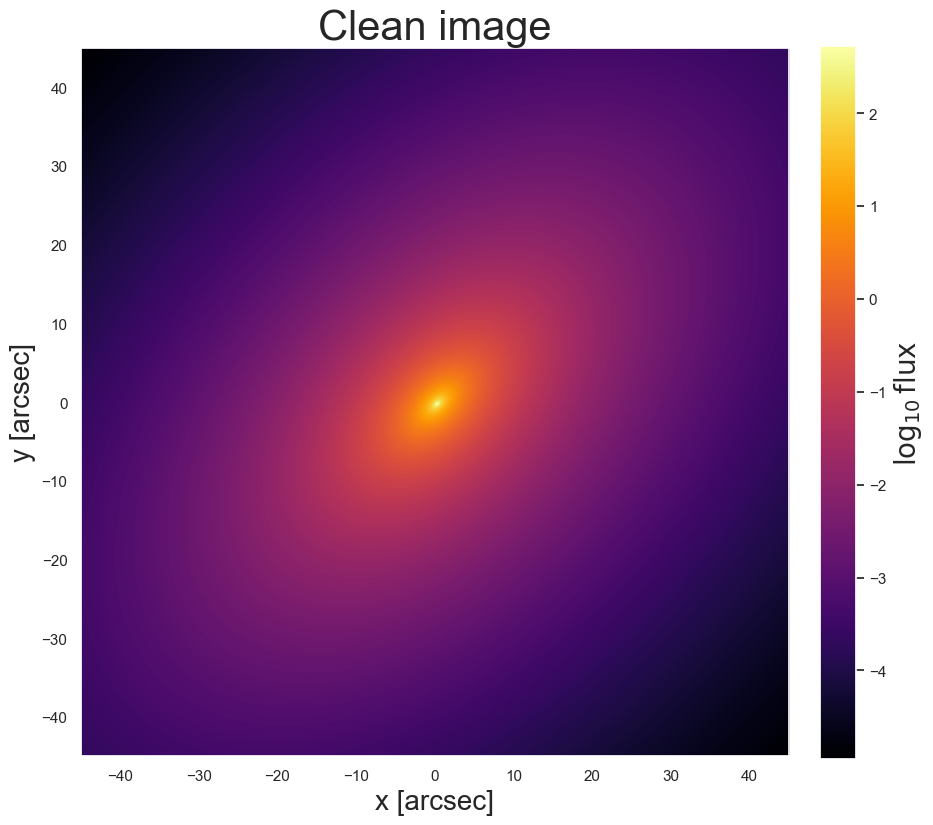
\includegraphics[width=0.75\linewidth, keepaspectratio]{img/chapter5/sersic/0_clean.png}\label{fig:0_clean}}
  \end{minipage}
  \begin{minipage}{\linewidth}
    \centering
    \subfloat[]{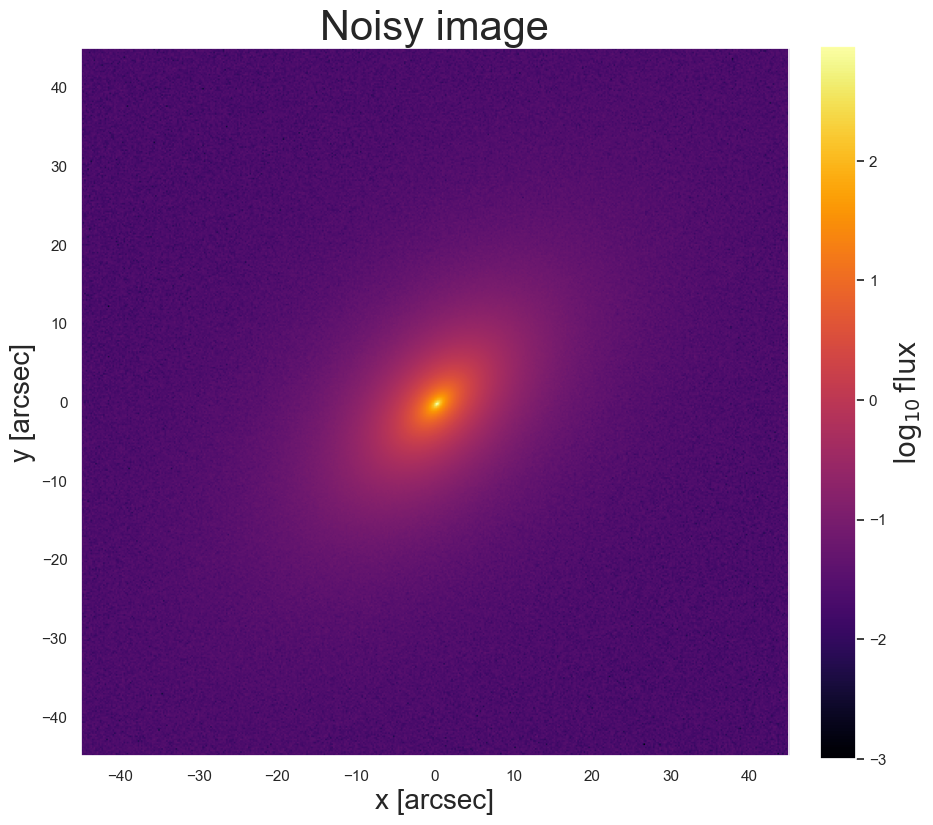
\includegraphics[width=0.75\linewidth, keepaspectratio]{img/chapter5/sersic/0_noisy.png}\label{fig:0_noisy}}
  \end{minipage}
  \caption[Simulated Sérsic surface brightness: theoretical + noisy]{Simulation of a galaxy with Sérsic surface brightness distribution: \protect\subref{fig:0_clean} theoretical model and \protect\subref{fig:0_noisy} image with Gaussian noise+PSF.}
  \label{fig:obs}
\end{figure}

\begin{figure}
    \centering
    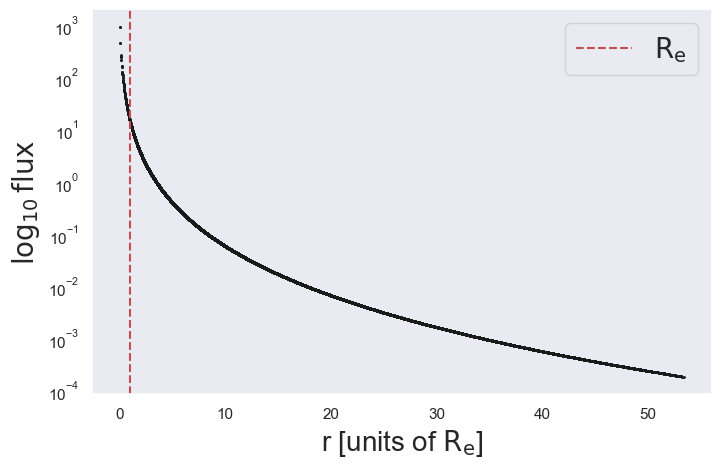
\includegraphics[width=0.8\linewidth, keepaspectratio]{img//chapter5/sersic/0_flux_r.png}
    \caption[Simulated Sérsic surface brightness vs radius]{Simulated Sérsic surface brightness distribution as a function of distance from the center of the galaxy, in units of the effective radius.}
    \label{fig:0_flux}
\end{figure}

\subsubsection{Fitting the model to data}

The next step involves fitting the model to the observational data. In this context, we establish a cost function and an optimizer, and we proceed by utilizing automatic differentiation frameworks such as PyTorch and TensorFlow. As discussed in \cref{chap:algorithms}, these components are tasked with quantifying the discrepancy between the theoretical model and the observed data and updating the model parameters by gradient descent, respectively. For this task, one of the most commonly used cost functions in regression problems, the Mean Squared Error\footnote{\url{https://pytorch.org/docs/stable/generated/torch.nn.MSELoss.html}.}\textsuperscript{,}\footnote{\url{https://www.tensorflow.org/api_docs/python/tf/keras/losses/MeanSquaredError}.} (MSE), was selected. The MSE is advantageous for its simplicity and effectiveness in quantifying the average squared discrepancy between the predicted and actual values. This makes it particularly suitable for regression tasks that aim to minimize the difference between predicted results and observed data \citep{berger_statistical_2006}.

Regarding the optimizer, Adam\footnote{\url{https://pytorch.org/docs/stable/generated/torch.optim.Adam.html}.}\textsuperscript{,}\footnote{\url{https://www.tensorflow.org/api_docs/python/tf/keras/optimizers/Adam}.} \citep{kingma_adam_2017} was chosen for its ability to combine the advantages of two other popular optimizers: AdaGrad and RMSProp \citep{tieleman_rmsprop_2014}. Adam stands out for its adaptive learning rate, which adjusts as training progresses, making it efficient for large-scale and complex problems. This adaptability is particularly beneficial for navigating complex high-dimensional data landscapes, often leading to faster convergence than other gradient descent methods.

In addition, a learning rate scheduler has been defined to improve the efficiency of model training by automatically adjusting the step $\eta$ taken by the optimizer in parameter updates\footnote{\url{https://pytorch.org/docs/stable/generated/torch.optim.lr_scheduler.ReduceLROnPlateau.html}.}\textsuperscript{,}\footnote{\url{https://www.tensorflow.org/api_docs/python/tf/keras/callbacks/ReduceLROnPlateau}.}. The initial learning rate for the optimizer is set to $\eta = 0.1$ and gradually decreases to improve the speed of finding the minimum loss function.

At this point, the model must be initialized with some initial (random) parameters that are appropriately constrained, shown in \cref{tab:parameters_1}.

\begin{table}[]
\setlength{\extrarowheight}{2pt}
\setlength{\tabcolsep}{1pt}
\centering
\caption{Summary of true and initial parameters before fitting.}
\label{tab:parameters_1}
%\resizebox{0.2\linewidth}{!}{
\begin{tabular}{@{}c@{\hskip 20pt}c@{}@{\hskip 20pt}c@{}}
\toprule
Parameter           & True value                 &  Initial value            \\ \midrule
$I_e$               & \SI{15.0}{}                &  \SI{25.0}{}              \\
$R_e$               & \SI{2.0}{\arcsecond}       &  \SI{4.5}{\arcsecond}     \\
$n$                 & \SI{5.5}{}                 &  \SI{7.0}{}               \\
$x_0$               & \SI{0.2}{\arcsecond}       &  \SI{12.2}{\arcsecond}     \\
$y_0$               & \SI{-0.3}{\arcsecond}      &  \SI{-18.0}{\arcsecond}    \\
$q$                 & \SI{0.6}{}                 &  \SI{0.8}{}               \\
$\varphi$           & \SI{0.7853}{\radian}       &  \SI{1.5708}{\radian}     \\ \bottomrule
\end{tabular}
%}
\end{table}

\begin{figure}[]
  \begin{minipage}{0.49\linewidth}
    \centering
    \subfloat[]{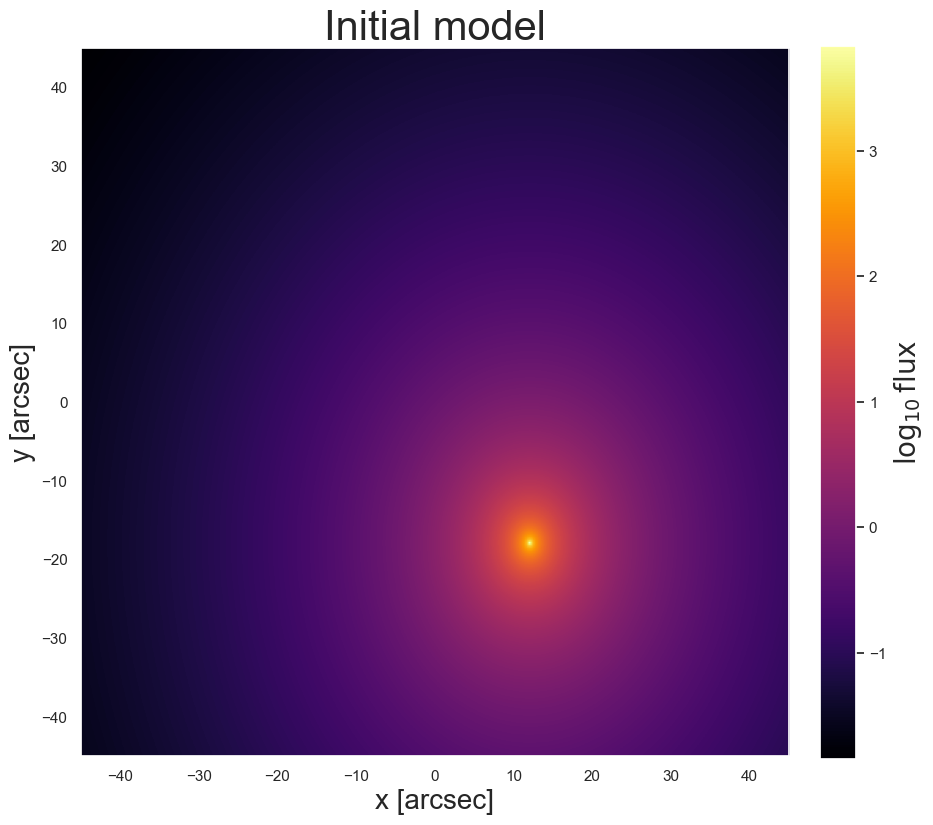
\includegraphics[width=\linewidth, keepaspectratio]{img/chapter5/sersic/1_initial.png}\label{fig:1_model_sersic}}
  \end{minipage}
  \begin{minipage}{0.49\linewidth}
    \centering
    \subfloat[]{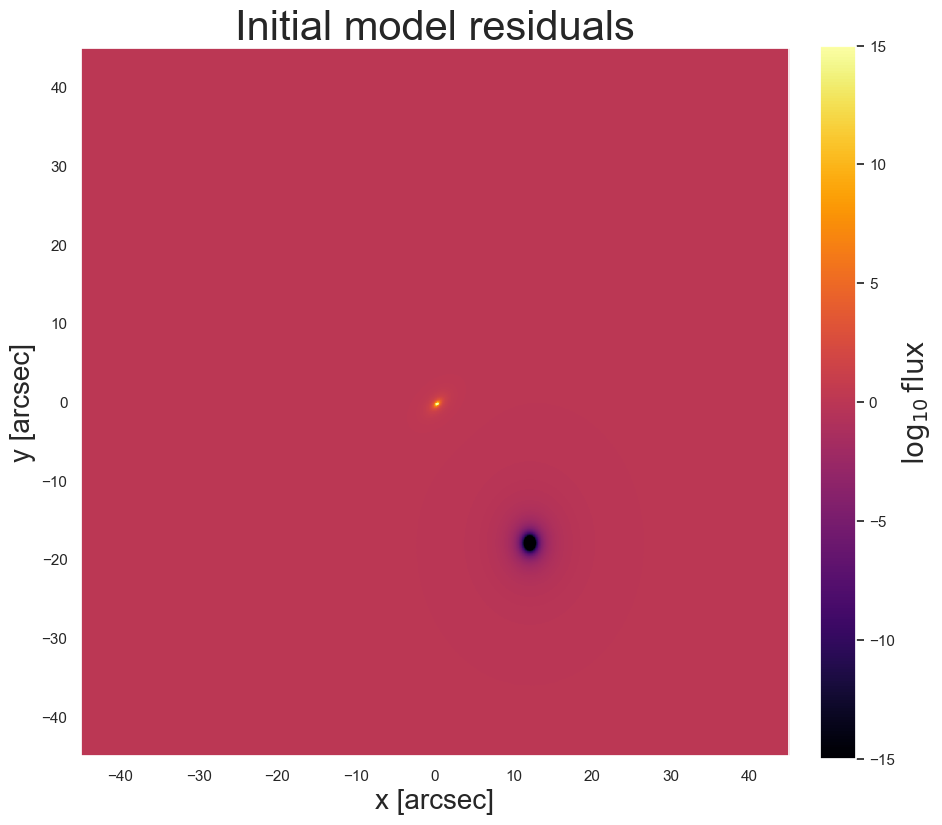
\includegraphics[width=\linewidth, keepaspectratio]{img/chapter5/sersic/1_residuals.png}\label{fig:1_model_residuals_init}}
  \end{minipage}
  \caption[Initial prediction Sérsic profile + residuals]{\protect\subref{fig:1_model_sersic} Initial prediction of Sérsic surface brightness model, computed using the initial values of \cref{tab:parameters_1} and \protect\subref{fig:1_model_residuals_init} residuals, normalized by their standard deviation, calculated as subtraction between true data and initial prediction.}
  \label{fig:1_initial}
\end{figure}

\begin{figure}
  \begin{minipage}{0.49\linewidth}
    \centering
    \subfloat[]{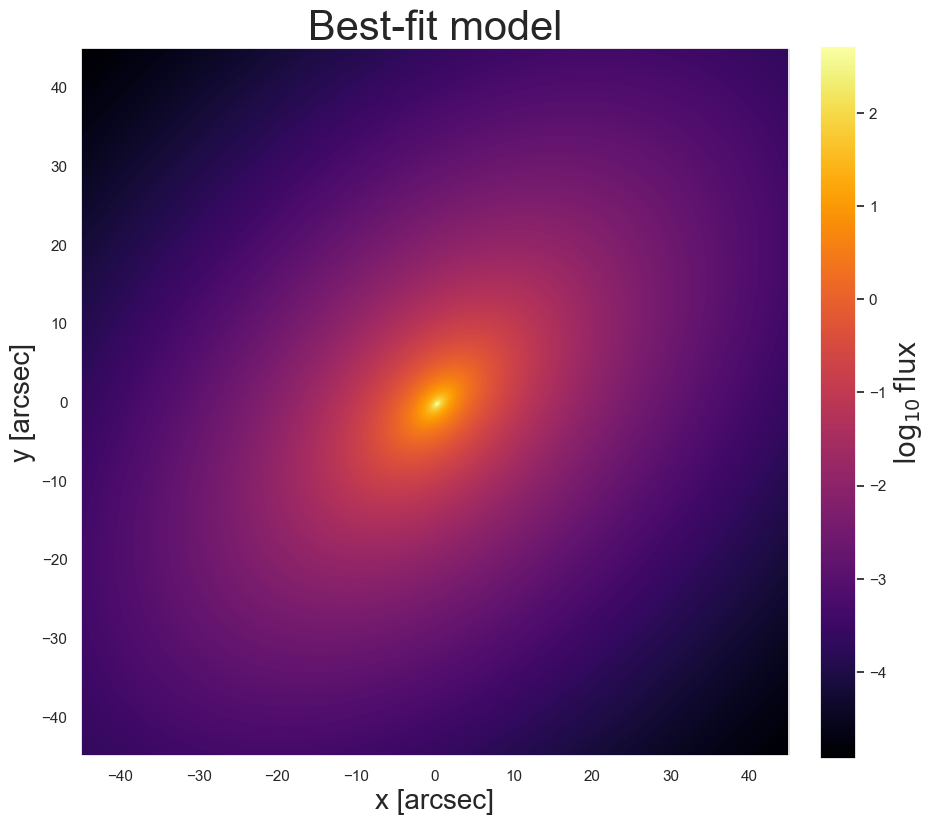
\includegraphics[width=\linewidth, keepaspectratio]{img/chapter5/sersic/sersic_best_fit.png}\label{fig:bestfit_sersic}}
  \end{minipage}
  \begin{minipage}{0.49\linewidth}
    \centering
    \subfloat[]{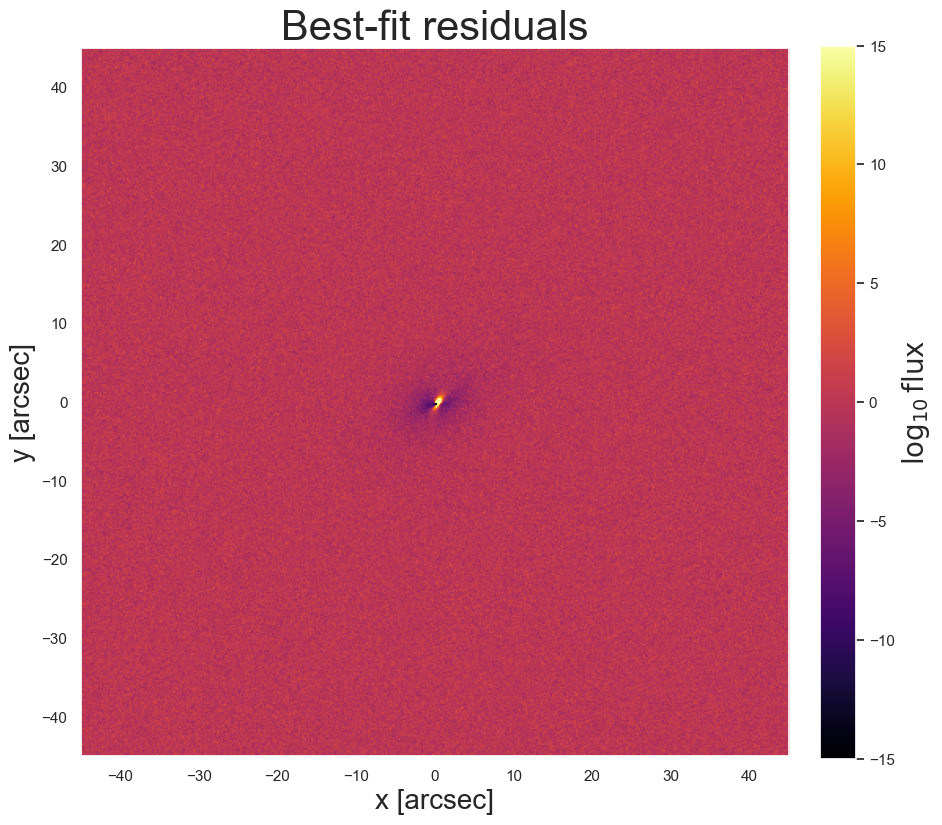
\includegraphics[width=\linewidth, keepaspectratio]{img/chapter5/sersic/res_bestfit.png}\label{fig:res_bestfit}}
  \end{minipage}
  \caption[Best-fit prediction Sérsic profile + residuals]{\protect\subref{fig:bestfit_sersic} Best-fit prediction of Sérsic surface brightness model, computed using the best-fit values of \cref{tab:parameters_2} obtained from the training process and \protect\subref{fig:res_bestfit} residuals normalized by their standard deviation, calculated as subtraction between true data and best-fit prediction.}
  \label{fig:sersic_best}
\end{figure}

The initial prediction of the model, accompanied by residuals for the actual data, is presented in \cref{fig:1_initial}. Subsequently, the model training can start. To speed up the fitting process, it is possible to minimize the cost function computed on the logarithms of the model and data as a way to normalize the data between a smaller range of values \citep{huang_normalization_2020}.

Before training the cost function, \ie the MSE between the data and the model has a value of $\mathrm{loss_{initial}} = 5.4$ and, after $50000$ iterations (or epochs) of the training loop, it drops to $\mathrm{loss_{final}} = 3.1\pwr{-10}$, reaching its absolute minimum. The best-fit parameters are reported in \cref{tab:parameters_2} and \cref{fig:loss_sersic} shows the trend of the MSE as a function of iterations of gradient descent.

\begin{figure}[]
    \centering
    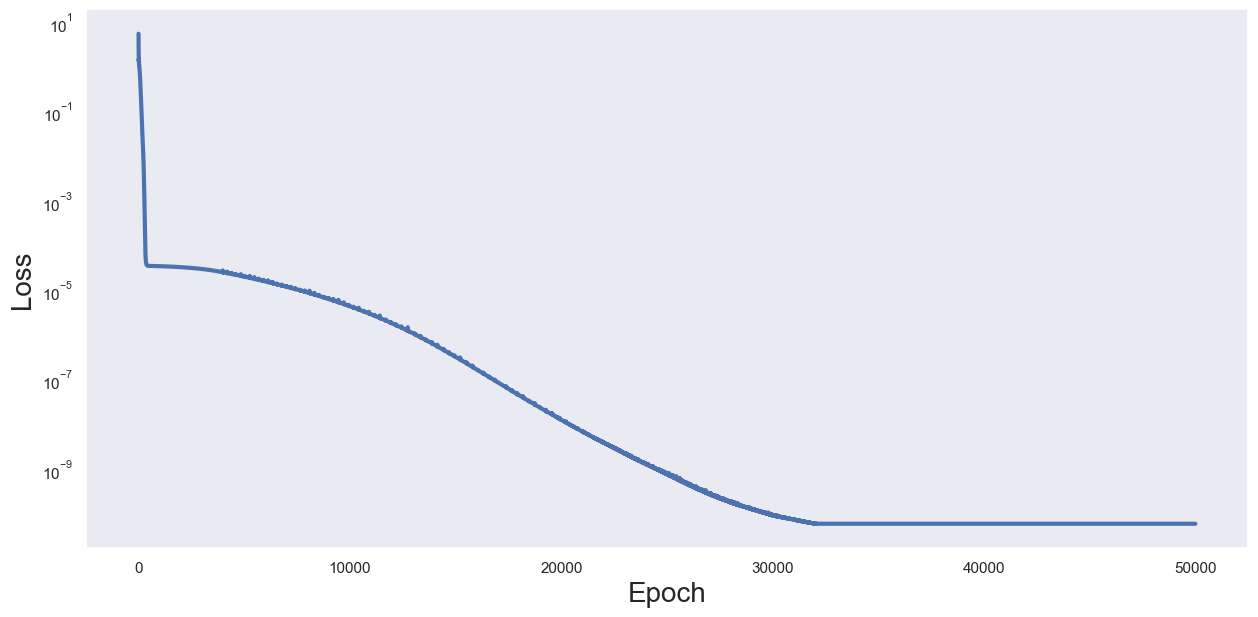
\includegraphics[width=\linewidth]{img//chapter5//sersic/loss_sersic.png}
    \caption[Loss function vs epochs for Sérsic profile fit]{Loss function vs epochs for the training of the Sérsic model.}
    \label{fig:loss_sersic}
\end{figure}

After training the model, an estimation of parameter errors was performed throughout MCMC sampling, using the Pyroframework. Pyro is a probabilistic programming language built on top of PyTorch, designed to create and run complex probabilistic models. It offers tools for defining flexible and expressive Bayesian models and algorithms for variational inference, making it well-suited for tasks in machine learning and statistics that involve uncertainty. Pyro's integration with PyTorch allows for automatic differentiation and GPU acceleration, enabling efficient and scalable model fitting and evaluation.

The probabilistic model was defined with a uniform distribution for the parameters, and then $5000$ samples from the posterior distributions were extracted. Their mean values and standard deviations are described in \cref{tab:parameters_2}.

\begin{table}[]
\setlength{\extrarowheight}{2pt}
\setlength{\tabcolsep}{1pt}
\centering
\caption{Summary of true, initial and best-fit parameters.}
\label{tab:parameters_2}
%\resizebox{0.2\linewidth}{!}{
\begin{tabular}{@{}c@{\hskip 20pt}c@{}@{\hskip 20pt}c@{}@{\hskip 20pt}c@{}@{\hskip 20pt}c@{}}
\toprule
Parameter   & True value            & Initial value             & Best-fit value            & Best-fit value (MCMC) \\ \midrule
$I_e$       & \SI{15.0}{}           & \SI{25.0}{}               & \SI{15.0077}{}            & \SI[separate-uncertainty=true]{14.9777 \pm 0.1499}{} \\
$R_e$       & \SI{2.0}{\arcsecond}  & \SI{4.5}{\arcsecond}      & \SI{1.9997}{\arcsecond}   & \SI[separate-uncertainty=true]{2.0014 \pm 0.0106}{\arcsecond} \\
$n$         & \SI{3.5}{}            & \SI{7.0}{}                & \SI{3.5002}{}             & \SI[separate-uncertainty=true]{3.5080 \pm 0.0376}{} \\
$x_0$       & \SI{0.2}{\arcsecond}  & \SI{12.2}{\arcsecond}     & \SI{0.2000}{\arcsecond}   & \SI[separate-uncertainty=true]{0.2000 \pm 0.0009}{\arcsecond}\\
$y_0$       & \SI{-0.3}{\arcsecond} & \SI{-18.0}{\arcsecond}    & \SI{-0.3000}{\arcsecond}  & \SI[separate-uncertainty=true]{-0.2999 \pm 0.0010}{\arcsecond}   \\
$q$         & \SI{0.6}{}            & \SI{0.8}{}                & \SI{0.5999}{}            & \SI[separate-uncertainty=true]{0.5999 \pm 0.0014}{}  \\
$\varphi$   & \SI{0.7853}{\radian}  & \SI{1.5708}{\radian}      & \SI{0.7854}{\radian}      & \SI[separate-uncertainty=true]{0.7854 \pm 0.0018}{\radian}\\ \bottomrule
\end{tabular}
%}
\end{table}

\Cref{fig:corner_sersic} shows the corner plot to illustrate the multidimensional distributions of and between the parameters. Diagonal elements consist of histograms representing the marginal distributions of individual parameters. They allow one to discern the central tendencies (such as mean or median), the spread (variance or standard deviation), and the shape (indications of skewness or multiple peaks) of each parameter's distribution. Off-diagonal elements display the joint distributions between pairs of parameters through contour plots. They are instrumental in understanding the correlations or dependencies between parameters, with circular patterns indicating minimal correlation and elongated ellipsoids suggesting strong correlations. The orientation of these ellipsoids further clarifies the nature of the relationship, be it positive or negative.

In particular, the corner plot shows the correlation between some parameters involved. As is known from the literature \citep{graham_concise_2005,ciotti_analytical_1999}, the Sérsic profile presents degeneracies between some of its parameters:
\begin{itemize}
    \item intensity $I_e$ and effective radius $R_e$: larger radius with lower intensity can produce a similar overall brightness as a smaller radius with higher intensity;
    \item Sérsic index $n$ and effective radius $R_e$: galaxies with higher Sérsic indices tend to also have larger effective radii, as both parameters are related to how light is distributed in a galaxy.
\end{itemize}
Additionally, \cite{trujillo_effects_2001,trujillo_effects_2001-1} showed that in addition to the intrinsic degeneracies among the Sérsic parameters, there are some further degeneracies between the latter and the PSF. One can think of the intrinsic galaxy axis ratio as a very intuitive example. The PSF is, by definition, rounder than a flattened galaxy; hence, its effect on the two-dimensional light distribution produces a rounder galaxy. The higher the FWHM in arcsecs, the rounder the observed galaxy is \citep{peng_detailed_2002,li_galaxy_2022}.

\begin{figure}
    \centering
    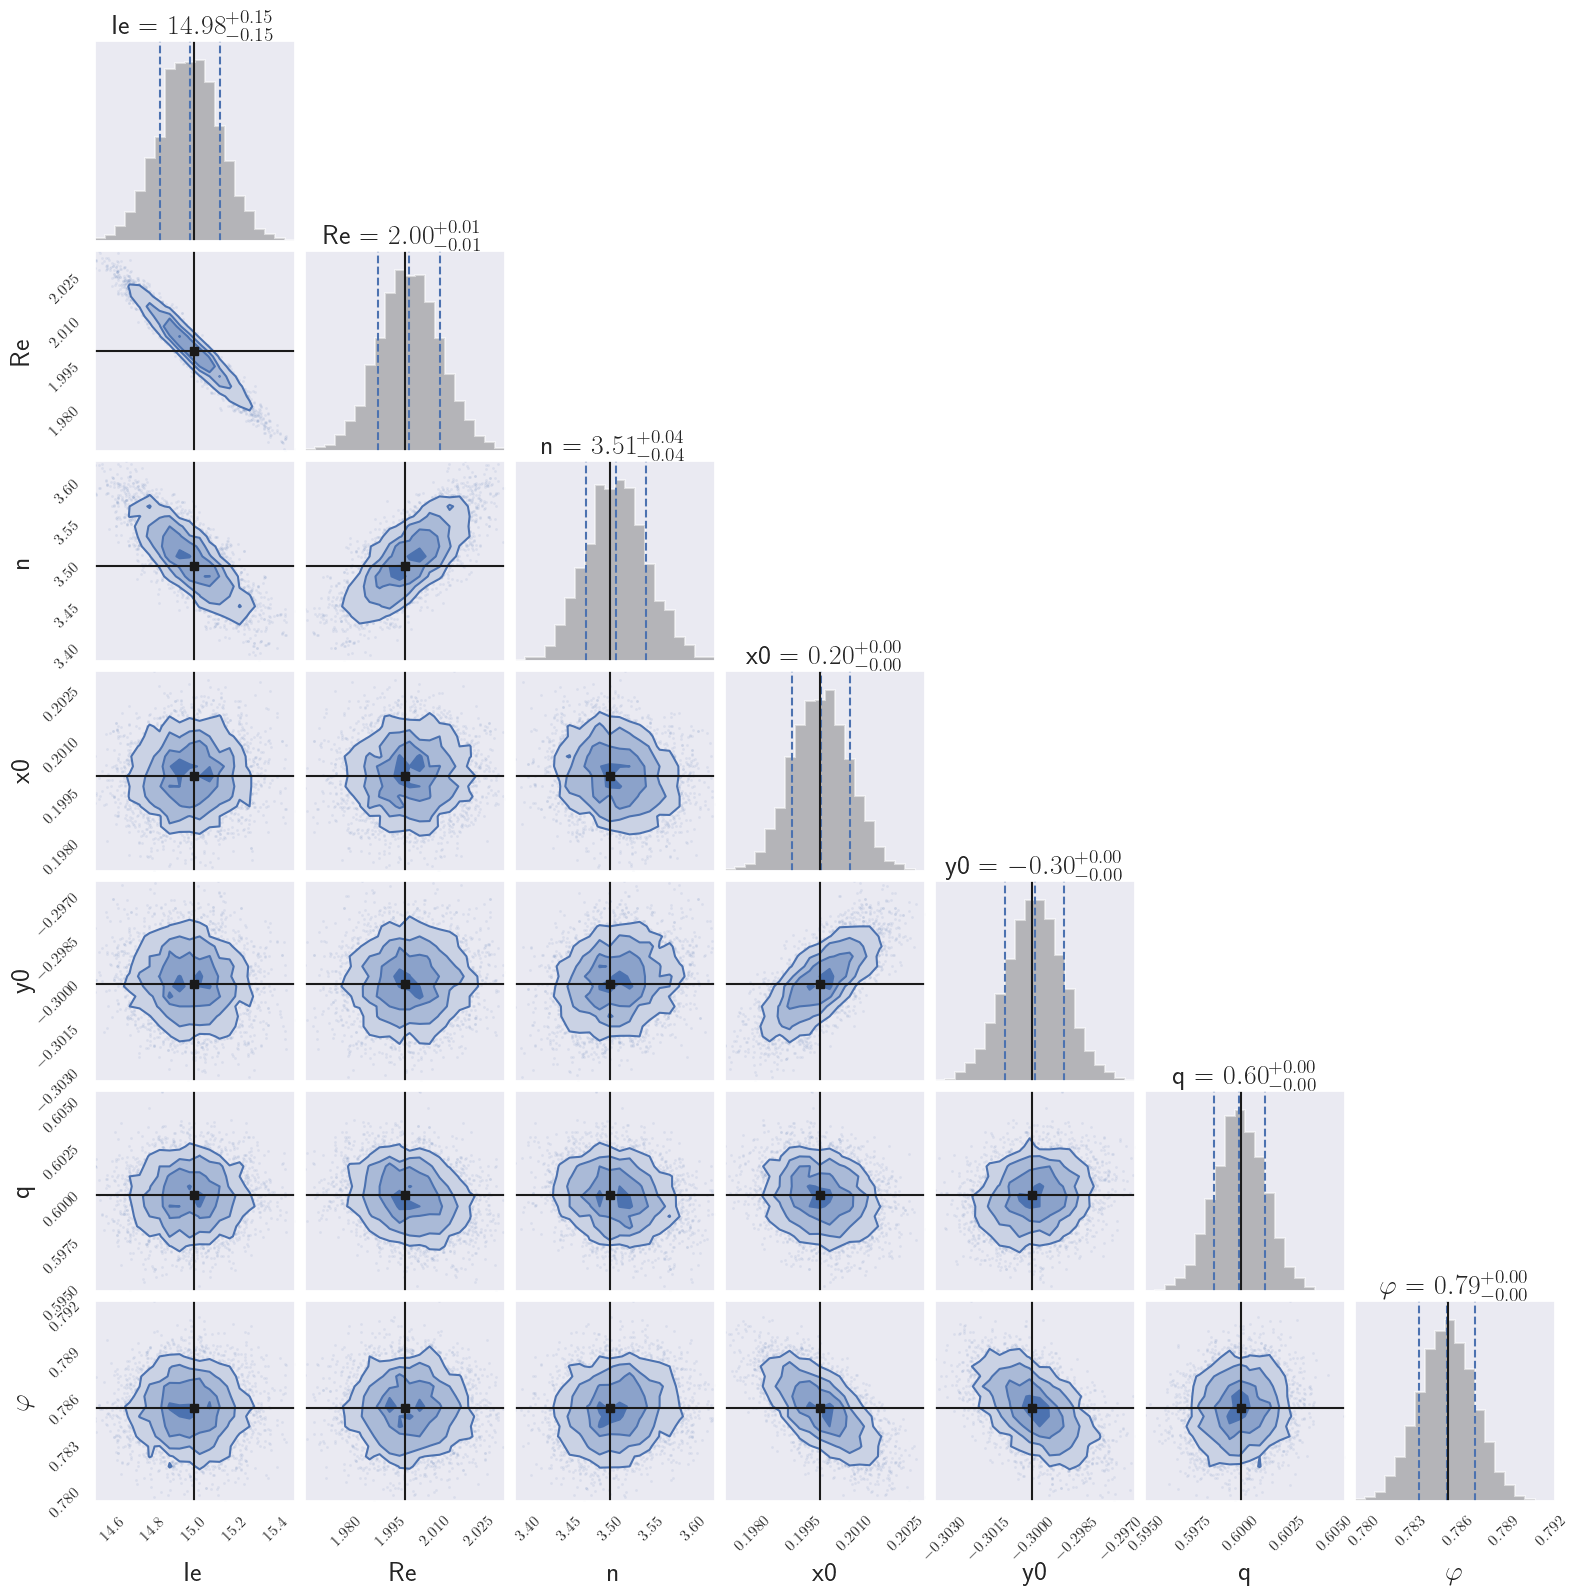
\includegraphics[width=\linewidth]{img//chapter5//sersic/corner_sersic.png}
    \caption[Corner plot Sérsic profile]{Corner plot showing the posterior probability distributions of the parameters used to fit the Sérsic surface brightness profile. The projections of the probability density on planes defined by each couple of parameters are shown, as well as one-dimensional marginalized distributions. The black and the blue dashed vertical lines in one-dimensional histograms indicate the true values and the 16th, 50th and 84th percentiles of the distributions.}
    \label{fig:corner_sersic}
\end{figure}